% =====================================================================
\section{The real LLM run with Google Gemini}\label{sec:gemini}
% =====================================================================

Every LLM result in Phases~4--7 came from the deterministic \emph{mock} provider, so the project could not claim
anything about LLM-driven discovery. After the project was assembled, a real provider for Google Gemini was added
and the Phase~6 pipeline was run with it.

\subsection{How the switch from mock to Gemini works}

\begin{itemize}
  \item \fn{config.yaml} sets \fn{llm.provider: "gemini"}. \fn{get_provider} returns a \fn{GeminiProvider} only
        if the environment variable \fn{GEMINI_API_KEY} is set; otherwise it warns and falls back to the mock.
  \item The key is read from the environment and never written anywhere. It lives in a local \fn{.env} file,
        which is listed in \fn{.gitignore}.
  \item \fn{experiments/11_real_llm_gemini.py} reuses the existing Phase~6 and Phase~7 code unchanged, refuses to
        run if the key is missing (so it can never silently use the mock), and writes only to
        \fn{results/evaluation/real_llm_gemini/}. The mock results were verified byte-for-byte unchanged.
\end{itemize}

\begin{figure}[!htb]
\centering
% flowchart 'gemini' -- used by docs/Report.tex
\begin{tikzpicture}[node distance=3.4mm and 7mm]
  \node[fnw=cExp] (main) {11_real_llm_gemini.main};
  \node[dec=cExp, below=of main] (key) {GEMINI_API_KEY\\set?};
  \node[fn=cExp, right=of key, font=\scriptsize] (stop) {stop: refuse to\\use the mock};
  \node[fnw=cLlm, below=of key] (gp) {get_provider $\to$ GeminiProvider\\{\normalfont\tiny model from the -{}-model flag or config}};
  \node[fnw=cExp, below=of gp] (sg) {stage_generate};
  \node[fnw=cExp, right=of sg] (rl) {09_evaluation.real_llm\\{\normalfont\tiny Mode A vs Mode B, 3 datasets}};
  \node[fnw=cExp, below=of sg] (p6) {_phase6_module\\{\normalfont\tiny load 08 script, redirect OUT}};
  \node[fnw=cExp, below=of p6] (st) {stage_prepare $\to$ stage_pinn\\$\to$ stage_select\\{\normalfont\tiny the unchanged Phase 6 stages}};
  \node[fnw=cExp, below=of st] (ar) {annotate_report};
  \node[fnw=cExp, below=of ar] (cm) {compare_with_mock};
  \node[io, below=of cm] (out) {results/evaluation/real\_llm\_gemini/};
  % provider internals
  \node[fnw=cLlm, right=of p6, yshift=-2mm] (gen) {GeminiProvider.generate};
  \node[fnw=cLlm, below=of gen] (cl) {_get_client\\{\normalfont\tiny lazy import of google.genai}};
  \node[fnw=cLlm, below=of cl] (gc) {models.generate_content\\{\normalfont\tiny JSON output mode}};
  \node[dec=cLlm, below=of gc] (err) {429/500/503?};
  \node[fnw=cLlm, below=of err] (rep) {_repair_json_escapes\\{\normalfont\tiny only if the JSON is invalid}};
  \begin{scope}[on background layer]
    \node[pkgbox=cLlm, fit=(gen)(cl)(gc)(err)(rep), label={[pkglabel=cLlm]below:inside every LLM call}] (box) {};
  \end{scope}
  \draw[flow] (main) -- (key); \draw[flow] (key) -- node[note, above]{no} (stop);
  \draw[flow] (key) -- node[note, right]{yes} (gp); \draw[flow] (gp) -- (sg); \draw[flow] (sg) -- (rl);
  \draw[flow] (sg) -- (p6); \draw[flow] (p6) -- (st); \draw[flow] (st) -- (ar); \draw[flow] (ar) -- (cm);
  \draw[flow] (cm) -- (out);
  \draw[flow] (gen) -- (cl); \draw[flow] (cl) -- (gc); \draw[flow] (gc) -- (err);
  \draw[flow] (err.east) -- node[note, above]{yes} ++(5mm,0) |- node[note, right, pos=0.25]{wait 5, 10, 20\ldots s} (gc.east);
  \draw[flow] (err) -- node[note, right]{no} (rep);
  \draw[dflow] (rl.south) -- (box.north -| rl.south);
\end{tikzpicture}

\pkglegend
\caption{The real-LLM run. Left: the runner reuses the existing stages. Right: what \fn{GeminiProvider.generate}
does on every call, including the two compatibility fixes added for Gemini.}
\label{fig:gemini}
\end{figure}

\subsection{Problems met, and the minimal fixes}

\begin{enumerate}
  \item \textbf{Overload.} The configured \fn{gemini-3.8-flash} (and \fn{gemini-3.5-flash}) repeatedly answered
        \emph{503: model is currently experiencing high demand}. The provider now retries 429/500/503 with
        increasing waits. When that was still not enough, the run used \fn{gemini-3.5-flash-lite}, passed with
        \fn{-{}-model} for that run only; the configuration was not changed.
  \item \textbf{Invalid JSON.} Gemini sometimes wrote \LaTeX{} such as \verb|\partial| inside JSON strings.
        That is an illegal escape, and the strict parser threw away the \emph{entire} response. The fix asks Gemini
        for its native JSON mode and, if the text still fails to parse, doubles stray backslashes.
\end{enumerate}
Neither fix touched the scientific pipeline. Many Gemini proposals were still (correctly) rejected by the project's
own validator, mostly because Gemini writes powers as \texttt{u\^{}3} where the compiler expects \texttt{u**3},
or uses $u_{xxxx}$, which is not in the derivative set.

\subsection{Results}

\textbf{Did evidence (RAG) change Gemini's hypotheses?} Yes, on all three test datasets.
\begin{center}
\small
\begin{tabular}{@{}p{2.8cm}p{5.6cm}p{5.6cm}@{}}
\toprule
\textbf{Dataset} & \textbf{Mode A (no evidence)} & \textbf{Mode B (with retrieved evidence)} \\ \midrule
diffusion & decay and logistic variants only; no plain diffusion & plain diffusion $u_t=D\,u_{xx}$ appears \\
reaction--diffusion & correct family $D\,u_{xx} + r\,u(1-u/K)$ & no valid hypothesis (one response failed schema) \\
advection--diffusion & correct family, velocity named $v$ & same family, renamed to the corpus's $c$ \\
\bottomrule
\end{tabular}
\end{center}

\textbf{Full Phase~6 pipeline with Gemini} (same data, splits and thresholds as the mock run):
\begin{center}
\small
\begin{tabular}{@{}>{\raggedright\arraybackslash}p{4.0cm}>{\raggedright\arraybackslash}p{5.4cm}>{\raggedright\arraybackslash}p{5.4cm}@{}}
\toprule
 & \textbf{Mock (Phase 6)} & \textbf{Gemini (gemini-3.5-flash-lite)} \\ \midrule
LLM candidates & $D\,u_{xx}$;\ $c\,u_x$ advection;\ reaction--diff.;\ adv.--diff. & $D\,u_{xx}$;\ $D\,u_{xx}-r\,u$;\ adv.--diff.;\ reaction--diff. \\
Graph templates added & K3 (pure reaction) & K1 (pure advection), K3 \\
Passed the gate & H1, H3, H4 & H1, H2, H3, H4 \\
Rejected & H2 (advection), K3 & K1 (advection), K3 \\
\textbf{Selected} & $u_t = D\,u_{xx}$ & $u_t = D\,u_{xx}$ \\
$\hat D$ (error) & 0.10002 (0.021\%) & 0.10001 (0.011\%) \\
Holdout RMSE & 0.01214 & 0.01218 \\
OOD RMSE, noisy obs. & 0.01144 & 0.01160 \\
OOD RMSE vs clean field (oracle) & 0.00181 & 0.00201 \\
Novel window $t\in(1,1.5]$ (oracle) & $2.5\times10^{-4}$ & $2.7\times10^{-4}$ \\
\bottomrule
\end{tabular}
\end{center}

Gemini's three more complex candidates all fit as well as diffusion, but their extra terms were judged inactive
($r\approx0.013$, $c\approx0.001$, $r\approx0.017$), each reduces to plain diffusion, and the same law won on
complexity and BIC. The real LLM proposed more physically plausible alternatives than the mock's canned pure
advection, and the pipeline reached the same, correct conclusion.

\begin{figure}[!htb]
\centering
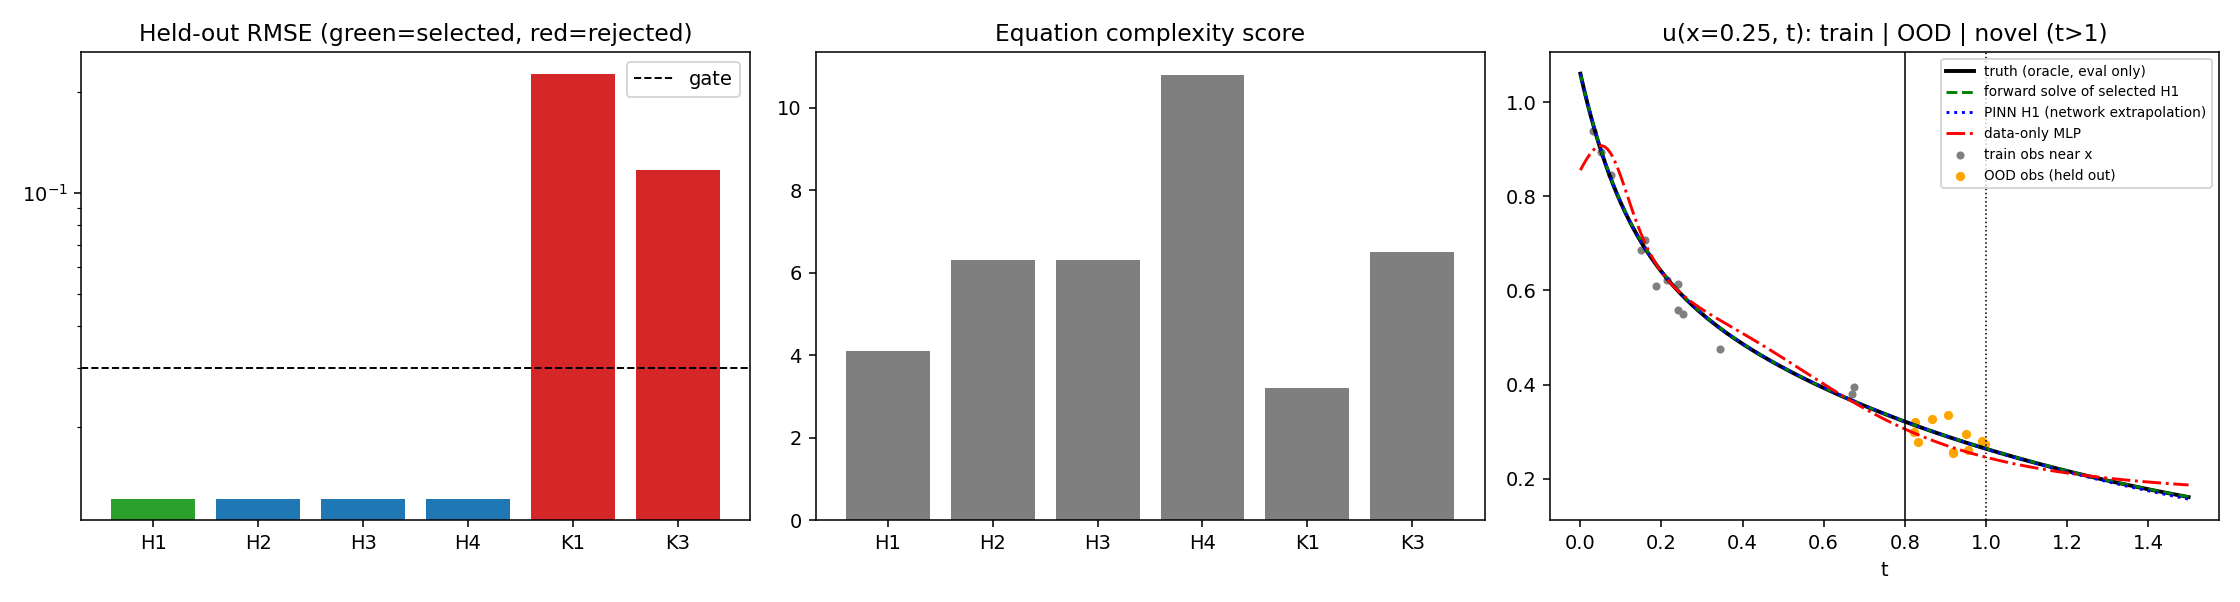
\includegraphics[width=\textwidth]{results/evaluation/real_llm_gemini/phase6/phase6_summary.png}
\caption{The Gemini run's Phase~6 summary (from \fn{results/evaluation/real_llm_gemini/phase6/}), in the same
layout as the mock run's figure.}
\end{figure}

\begin{caution}[: one sample]
LLM output is random from run to run. This is a single Gemini sample on one dataset; it shows the pipeline works
with a real LLM and that evidence changes the proposals, not that Gemini reliably discovers laws.
\end{caution}

% =====================================================================
\section{What is and is not demonstrated}\label{sec:limits}
% =====================================================================

The project's final report audits every claim. In short:
\begin{center}
\small
\begin{tabular}{@{}p{4.2cm}p{3.2cm}p{7.2cm}@{}}
\toprule
\textbf{Claim} & \textbf{Verdict} & \textbf{Why} \\ \midrule
PINN forward and inverse & demonstrated & $D$ and $c$ recovered within 0.4\% on two systems \\
Physics-constrained search & demonstrated & Phase~6 and the second system \\
OOD and novel prediction & demonstrated & both systems; physics-free network 6--40$\times$ worse \\
Adversarial robustness & demonstrated & 20/20 (3 by abstention) \\
LLM-driven discovery & partial (new) & one real Gemini run; same correct answer as the mock \\
RAG contribution & partial & recall only; top-1 retrieval 1/6 \\
Knowledge-graph contribution & partial & structured queries and provenance; no accuracy gain \\
Noisy-data robustness & partial & PINN path works at 5\% noise; SINDy fails \\
Uncertainty & partial & bootstrap only, not Bayesian; disagrees with the PINN on H3 \\
Equation uniqueness & not demonstrated & nested models fit equally; selection is a stated parsimony rule \\
Boundary/initial-condition inference & not demonstrated & supplied as known physics \\
Real-world data; a new law & not demonstrated & synthetic 1D data; known laws recovered \\
\bottomrule
\end{tabular}
\end{center}

\textbf{Main limitations.} Synthetic one-dimensional PDEs only; boundary and initial conditions are given, not
inferred; lexical (word-hashing) retrieval over a five-document corpus; hand-set thresholds (fixed in advance, but
not calibrated on independent data); the fast regression engine has no noise robustness; and uncertainty is a
bootstrap, not a posterior.

% =====================================================================
\section{Glossary}
% =====================================================================

\begin{description}[style=nextline, itemsep=1pt, font=\normalfont\bfseries]
  \item[Ablation] Removing one component at a time to measure how much it contributes.
  \item[Abstention] Declining to select any law when no candidate passes the gate. Safe, but not discovery.
  \item[Autograd] Automatic, exact differentiation of a neural network's output, used for $u_t, u_x, u_{xx}$ in PINNs.
  \item[BIC] Bayesian information criterion, $n\ln(\mathrm{MSE}) + k\ln n$: fit quality plus a penalty per parameter.
  \item[Canonical signature] An equation's structure with parameter names and signs normalised, for duplicate detection.
  \item[Collocation points] Random $(x,t)$ points where a PINN's equation residual is penalised; no data is needed there.
  \item[Complexity score] Terms + free parameters + derivative order + 2$\times$nonlinear terms + 0.1$\times$operations.
  \item[Embedding] A vector representing a piece of text, so similar texts get similar vectors.
  \item[Finite differences] Approximating derivatives from neighbouring grid values; amplifies noise.
  \item[Forward / inverse problem] Forward: parameters known, predict $u$. Inverse: estimate unknown parameters from data.
  \item[Gate] The pass/fail check on held-out error, physics residual, BC, IC and physical bounds.
  \item[Hypothesis] A candidate equation with its unknown parameters, in the \fn{Hypothesis} JSON schema.
  \item[Identifiability] Whether the data can distinguish two terms at all (the eigenfunction trap is a failure of it).
  \item[Knowledge graph] Typed entities and typed relationships, each with provenance.
  \item[Leakage] Any route by which the hidden answer could influence a decision.
  \item[Nested model] A model that contains another as a special case (reaction--diffusion with $r=0$ is diffusion).
  \item[OOD] Out-of-distribution: here, observations later than $t=0.8$ that no decision ever sees.
  \item[Oracle] The hidden truth, used only to report error after all decisions.
  \item[PINN] Physics-informed neural network: a network trained to fit data and obey an equation.
  \item[RAG] Retrieval-augmented generation: retrieve relevant documents and include them in the LLM prompt.
  \item[Residual] For an equation written as $\mathcal{R}=0$, the value of $\mathcal{R}$; zero when the equation holds.
  \item[SINDy / STLSQ] Sparse regression for equation discovery / its thresholded least-squares solver.
  \item[Term necessity] The share of $u_t$ a parameter's terms contribute; under 5\% means inactive.
\end{description}
